\documentclass[12pt,a4paper]{article}
\usepackage[utf8]{inputenc}
\usepackage{times}
\usepackage{amsmath}
\usepackage{amssymb}
\usepackage{graphicx}
\usepackage{cite}
\usepackage{url}
\usepackage{hyperref}
\usepackage{geometry}
\usepackage{setspace}
\usepackage{indentfirst}
\usepackage{fancyhdr} % For page numbers
\usepackage[font={it,footnotesize}]{caption} % For caption formatting (10pt)
\usepackage{sectsty} % For section title formatting
\usepackage{booktabs} % For professional quality tables
\usepackage{tikz}
\usetikzlibrary{shapes.geometric, arrows, positioning, fit, calc}

% Set section/subsection title format (12pt, bold)
\sectionfont{\fontsize{12}{15}\selectfont\bfseries}
\subsectionfont{\fontsize{12}{15}\selectfont\bfseries}

% Set page number to bottom center
\pagestyle{fancy}
\fancyhf{}
\fancyfoot[C]{\thepage}
\renewcommand{\headrulewidth}{0pt}

% Set page margins
\geometry{left=2.54cm,right=2.54cm,top=2.54cm,bottom=2.54cm}

% Set line spacing to 1.5
\renewcommand{\baselinestretch}{1.5}

% Set paragraph indentation
\setlength{\parindent}{0.5cm}

% Title formatting
\title{\fontsize{14}{17}\selectfont\textbf{Advances in Deep Learning for Remote Sensing Image Classification: A Comprehensive Review}}
\author{Liang Jingyu\\
Northwestern Polytechnical University\\
Xi'an, Shaanxi, China\\
\texttt{3445078775@qq.com}}
\date{}

\begin{document}

\maketitle

\begin{abstract}
The application of deep neural networks has profoundly altered the landscape of Earth observation image analysis, where advanced layered architectures now yield remarkable accuracy. Their success in complex tasks such as scene interpretation, object localization, and fine-grained semantic segmentation is largely driven by refined techniques for multi-scale representation learning, the integration of adaptive attention mechanisms to weight salient features, and strategic parameter transfer across different domains. Nevertheless, the field still grapples with several persistent obstacles. A significant challenge lies in the scarcity of extensively labeled datasets, which is compounded by substantial computational overhead that can limit deployment on resource-constrained platforms. Furthermore, ensuring models are robustly adapted to diverse atmospheric, seasonal, and sensor-specific variations remains a critical area of focus. In response to these issues, a number of promising research trajectories are gaining momentum, including self-supervised pretraining on vast unlabeled archives and the synergistic fusion of multi-modal data streams like spectral and temporal information. Concurrently, the development of compact yet powerful network architectures is crucial for enhancing efficiency, thereby opening tangible paths for methodological innovation in this swiftly progressing area.
\end{abstract}

\textbf{Keywords:} Deep learning, Remote sensing, Image classification, Convolutional neural networks, Scene classification, Object detection

\section{Introduction}
\label{sec:introduction}

Recent years have witnessed a profound evolution in remote sensing, marked by the deployment of integrated space, air, and ground observation networks. These coordinated platforms are now generating an unprecedented deluge of high-resolution imagery. Imbued with a wealth of spectral, spatial, and temporal details, this data provides an indispensable foundation for a diverse array of applications, from land cover analysis and urban planning to disaster response and environmental stewardship. This explosion of information, however, also presents a formidable challenge. The sheer volume and intricate nature of modern remote sensing data have begun to outstrip the capabilities of conventional classification techniques, creating a clear need for more powerful analytical methods.

\begin{table}[htbp]
\centering
\caption{Overview of Deep Learning Applications in Remote Sensing}
\label{tab:applications}
\begin{tabular}{@{}lll@{}}
\toprule
\textbf{Application} & \textbf{Primary Task} & \textbf{Key Challenge} \\ 
\midrule
Scene Classification & Image-level labeling & Multi-scale features \\
Object Detection & Localization \& recognition & Small object detection \\
Semantic Segmentation & Pixel-level classification & Class imbalance \\
\bottomrule
\end{tabular}
\end{table}

Historically, approaches to remote sensing image classification were centered on features designed by hand. Analysts would meticulously engineer identifiers based on spectral signatures, textural patterns, or geometric properties. While such methods proved valuable for certain well-defined tasks, their effectiveness often diminishes when confronted with the high dimensionality and complexity of modern datasets. These engineered features frequently struggle to capture the intricate, non-linear relationships inherent in the data, especially when encountering diverse land cover classes or inconsistent imaging conditions \cite{cheng2016survey}. Moreover, the manual feature engineering process is notoriously labor-intensive and demands substantial domain expertise, a dependency that severely hampers the adaptability of these traditional methods to new sensor technologies and application domains.

The advent of deep learning has brought about a paradigm shift in computer vision, opening up new frontiers for the analysis of remote sensing imagery \cite{zhu2017deep}. In a departure from traditional machine learning paradigms, deep learning frameworks can autonomously discern and learn hierarchical feature representations directly from raw pixel data. This capability obviates the laborious process of manual feature engineering. Within the deep learning arsenal, convolutional neural networks (CNNs) have emerged as particularly powerful, demonstrating exceptional classification performance by adeptly capturing the spatial patterns and contextual nuances inherent in image data.

Following these advancements, researchers have increasingly adapted CNNs for remote sensing image classification, yielding substantial gains in both accuracy and operational robustness \cite{liu2019learning}. Yet, remote sensing data possesses distinct characteristics that differentiate it from natural imagery, such as numerous spectral bands, variable spatial resolutions, intricate scene compositions, and often a scarcity of labeled training examples \cite{cheng2016survey}. Confronting these unique properties has spurred the creation of specialized CNN architectures and innovative training strategies tailored specifically to the demands of remote sensing applications.

This paper presents a thorough review of the progress made in deep learning for remote sensing image classification, with a specific focus on innovations emerging between 2020 and 2023. We explore significant improvements related to CNN architectures, refined training methodologies, and specific adaptations for various applications. The discussion is structured to first provide essential background on the fundamental concepts of applying CNNs to remote sensing in Section 2. Subsequently, Section 3 examines recent architectural developments. Section 4 then shifts to three principal application domains: scene classification, object detection, and semantic segmentation. The review proceeds in Section 5 with a discussion of prevailing challenges and potential avenues for future research, before culminating in Section 6 with a summary of the principal findings.

\section{Background}
\label{sec:background}

\subsection{Convolutional Neural Networks Fundamentals}
Convolutional neural networks represent a class of deep learning architectures that are meticulously engineered for processing data with a grid-like topology, such as imagery. A typical CNN is composed of several fundamental building blocks, including layers for convolution, pooling, and fully connected operations, as well as activation functions that introduce non-linearity.

The convolutional layers serve as the feature extractors of the network. They apply a series of learnable filters across the input image, with each filter specialized to detect local patterns like edges, textures, or shapes. These convolutional operations offer two key efficiencies: parameter sharing, which dramatically reduces the total number of trainable weights, and local connectivity, which allows the model to effectively learn spatial hierarchies. Following convolution, pooling layers are commonly used to downsample the feature maps. This process reduces spatial dimensions while retaining the most salient information, which in turn makes the network more resilient to minor input translations and less computationally demanding. The general architectural framework often employed in remote sensing is depicted in Figure~\ref{fig:architecture}.

After several stages of convolution and pooling, the resulting high-level feature representations are passed to fully connected layers. These layers integrate the extracted features to perform the final prediction, whether it be a classification or regression task. Throughout the network, activation functions are interspersed to introduce non-linear transformations. This non-linearity is critical, as it empowers the network to model complex, non-linear relationships between its inputs and outputs. Among the most widely used activation functions are the Rectified Linear Unit (ReLU), sigmoid, and hyperbolic tangent (tanh).

\subsection{CNN Training and Optimization}
The training of a convolutional neural network centers on minimizing a loss function, which serves to quantify the discrepancy between the model's predictions and the actual ground truth labels. This optimization is typically accomplished through the backpropagation algorithm in conjunction with a gradient-based optimizer, such as stochastic gradient descent (SGD) or Adam.

Several techniques are commonly employed to improve CNN training performance and prevent overfitting, including:
\begin{itemize}
\item \textbf{Data augmentation}: Artificially expanding the training dataset through transformations such as rotation, scaling, and flipping
\item \textbf{Regularization}: Adding constraints to the loss function, such as L1/L2 regularization or dropout, to prevent overfitting
\item \textbf{Batch normalization}: Normalizing layer inputs to reduce internal covariate shift and accelerate training
\item \textbf{Transfer learning}: Utilizing pre-trained models from large-scale datasets and fine-tuning them for specific tasks
\end{itemize}

\subsection{Challenges in Remote Sensing Image Classification}
Remote sensing images present several unique challenges that distinguish them from natural images \cite{zhu2017deep}:

\begin{itemize}
\item \textbf{Multi-spectral information}: Remote sensing images often contain multiple spectral bands beyond RGB, requiring adaptation of CNN architectures to handle additional channels
\item \textbf{Varying spatial resolutions}: Different sensors capture images at different spatial resolutions, affecting the scale of objects and features \cite{cheng2016survey}
\item \textbf{Complex scene compositions}: Remote sensing scenes typically contain multiple objects with complex spatial relationships and varying scales \cite{xia2017aid}
\item \textbf{Limited labeled data}: Acquiring accurately labeled remote sensing data is expensive and time-consuming, leading to small training datasets \cite{zhu2017deep}
\item \textbf{Class imbalance}: Certain land cover classes may be significantly underrepresented in the training data
\end{itemize}

These challenges have motivated the development of specialized CNN architectures and training strategies specifically designed for remote sensing applications, as discussed in the following sections.

\section{Developments in CNN Architectures for Remote Sensing}
\label{sec:developments}

\subsection{Multi-scale Feature Extraction}
A fundamental characteristic of remote sensing imagery is its multi-scalar nature, encompassing objects that range from small, discrete buildings to vast landscape features. This inherent property poses a significant challenge for conventional CNN architectures, which often rely on fixed-size receptive fields and can therefore struggle to effectively capture features across such a broad spectrum of scales. Consequently, a considerable amount of recent research has focused on developing methods that explicitly incorporate multi-scale feature extraction capabilities.

One successful strategy has been the integration of pyramid pooling modules. These modules work by applying several pooling operations in parallel at different spatial scales and then concatenating the resulting feature maps, which enables the network to simultaneously apprehend both fine-grained local details and broader global context. In a similar vein, atrous spatial pyramid pooling utilizes dilated convolutions set at various rates. This approach effectively expands the receptive field to gather information from larger areas without incurring the cost of additional computational resources.

Feature pyramid networks, by contrast, introduce a different architectural solution. They build a rich feature hierarchy by creating a top-down pathway with lateral connections that merges semantically strong, high-level features with spatially precise, low-level features. The result is a feature pyramid that is semantically rich at every level, substantially improving the network's capacity for detecting objects of widely varying sizes.

\subsection{Attention Mechanisms}
Attention mechanisms have gained significant traction within the remote sensing community, as they provide a powerful means for neural networks to selectively focus on the most informative features and regions within an image. Broadly, these mechanisms can be classified into two primary types: spatial attention and channel attention.

The purpose of a spatial attention module is to generate a weighting map that highlights salient spatial locations within the feature maps. By doing so, these modules guide the network to concentrate on discriminative foreground objects while effectively suppressing interference from irrelevant background clutter. In parallel, channel attention modules are designed to model the interdependencies that exist between different feature channels. Their function is to adaptively re-calibrate channel-wise feature responses, thereby emphasizing channels that carry the most useful information and down-weighting those that are less pertinent to the task.

More advanced approaches, such as the convolutional block attention module, combine both spatial and channel-based attention mechanisms sequentially. This integration yields a more comprehensive and powerful attention capability. The inclusion of such modules has been demonstrated to yield notable improvements in classification accuracy, proving especially beneficial when analyzing complex remote sensing scenes that contain a multitude of object categories.

\subsection{Transfer Learning and Domain Adaptation}
The scarcity of labeled training data in many remote sensing applications has spurred considerable research into transfer learning and domain adaptation methodologies \cite{zhu2017deep}. The core idea of transfer learning is to harness the knowledge encapsulated in models trained on vast, general-purpose datasets, such as ImageNet, and repurpose it for specific remote sensing tasks.

A now-standard practice in remote sensing image classification is the fine-tuning of pre-trained CNN models. This procedure involves initializing a network with weights learned from a large-scale source dataset and then continuing the training process on the smaller, target remote sensing dataset. This approach consistently outperforms training a model from random initialization, particularly in scenarios where labeled data is scarce.

Domain adaptation techniques specifically tackle the distributional shift, or "domain gap," that often exists between generic natural images and specialized remote sensing data. To bridge this gap, various methods have been developed to align the feature distributions of the source and target domains. These techniques, which often employ adversarial training or explicit discrepancy minimization, facilitate a more effective and seamless transfer of knowledge from one domain to another.

\subsection{Lightweight Network Designs}
Computational efficiency is rapidly becoming a paramount concern in remote sensing, driven by the increasing need to deploy models on resource-limited platforms like satellites and unmanned aerial vehicles. In response, a significant area of research is dedicated to creating lightweight network designs that drastically reduce computational demands without a commensurate drop in classification accuracy.

One of the most effective techniques for achieving this is the use of depthwise separable convolutions. This operation refactors a standard convolution into two smaller steps: a depthwise convolution and a subsequent pointwise convolution. This decomposition dramatically curtails the overall computational complexity. Architectures like MobileNet and its successors have successfully leveraged this principle to deliver highly efficient performance, making them suitable for mobile and embedded device applications.

Another promising frontier is the application of neural architecture search (NAS). Instead of relying on human intuition, NAS algorithms can autonomously discover optimal network architectures tailored for specific remote sensing tasks. These automated approaches are capable of optimizing for multiple objectives, such as hardware constraints and performance metrics. In many cases, this process uncovers novel and highly efficient designs that surpass the performance of even meticulously handcrafted architectures.

\section{Application Cases}
\label{sec:applications}

This section reviews three major application areas where deep learning has been successfully applied. A summary of these tasks, their common architectures, and key challenges is provided in Table~\ref{tab:task_comparison}.

\begin{table}[h!]
\centering
\caption{Comparison of Major Deep Learning Tasks in Remote Sensing.}
\label{tab:task_comparison}
\resizebox{\textwidth}{!}{%
\begin{tabular}{@{}llll@{}}
\toprule
\textbf{Task} & \textbf{Description} & \textbf{Common Architectures} & \textbf{Key Challenges} \\ \midrule
Scene Classification & Categorize an image based on its overall content. & CNNs with global average pooling, Multi-scale networks & Intra-class diversity, Inter-class similarity \\
Object Detection & Locate and identify specific objects (e.g., vehicles). & Faster R-CNN, YOLO, SSD, Rotated BBox methods & Small object sizes, Varying orientations, Dense objects \\
Semantic Segmentation & Assign a class label to every pixel in an image. & FCN, U-Net, DeepLab, Encoder-Decoder models & Fine detail preservation, Class imbalance, Edge refinement \\ \bottomrule
\end{tabular}%
}
\end{table}


\subsection{Scene Classification}
Scene classification, a core task in remote sensing, involves assigning a semantic label to an entire image based on its predominant land use or land cover type. This endeavor is inherently difficult due to the complex compositional nature of remote sensing scenes, which often contain a heterogeneous mix of objects arranged in varied spatial configurations \cite{xia2017aid}.

Recent breakthroughs in scene classification have largely concentrated on developing models that can effectively capture both the overarching global context and the finer local object details \cite{zeng2018improving}. While global context features provide a holistic understanding of the scene's layout and general land cover distribution, local object features offer granular information about the specific, individual elements that constitute the scene.

To better integrate these different levels of information, multi-scale feature fusion approaches have become prevalent. These methods are designed to combine features that have been extracted at various spatial resolutions, thereby improving overall classification accuracy. Architecturally, this is often achieved through the use of feature pyramid structures or by employing parallel convolutional pathways with differently sized receptive fields, allowing the model to process both fine-grained details and coarse-grained context simultaneously.

Furthermore, attention mechanisms have been widely adopted in scene classification models. Their primary function is to enable the network to dynamically focus on the most discriminative regions within a complex scene. By helping to filter out irrelevant background noise and placing emphasis on the most informative areas, these mechanisms significantly contribute to a more robust and accurate understanding of the scene's content.

\subsection{Object Detection}
Object detection in remote sensing images involves locating and identifying specific objects such Object detection in the context of remote sensing requires both the precise localization and the accurate identification of specific items of interest, such as individual buildings, vehicles, or aircraft \cite{cheng2016survey}. The task is made particularly demanding by several factors inherent to overhead imagery, including the often diminutive size of target objects, their wide range of possible orientations, and the presence of cluttered, complex backgrounds \cite{zhang2016weakly}.

The methodologies for object detection can generally be divided into two main families. Two-stage methods, exemplified by frameworks like Faster R-CNN, first generate a set of candidate region proposals and subsequently classify each proposal. While these methods are known for achieving a high degree of accuracy, their multi-step nature can render them computationally burdensome, especially when applied to very large remote sensing images \cite{deng2017enhanced}.

In contrast, single-stage object detectors such as YOLO and SSD provide a more streamlined alternative. These models perform localization and classification in a single, unified pass through the network, which results in a significant boost in computational efficiency. To make these methods effective for remote sensing, researchers have introduced numerous adaptations, including the integration of multi-scale feature pyramids and the design of anchor boxes specifically optimized for the unique aspect ratios and sizes of objects found in aerial imagery.

A further layer of complexity is addressed by orientation-aware object detection methods. These approaches are explicitly designed to handle the challenge of objects appearing at arbitrary rotations, a common occurrence in top-down imagery. By directly incorporating orientation estimation into the detection framework, often through the use of rotated bounding boxes or dedicated angle prediction modules, these models can achieve substantially improved detection accuracy for non-upright objects.

\subsection{Semantic Segmentation}
Semantic segmentation aims to produce highly detailed land cover maps by assigning a specific class label to every individual pixel within a remote sensing image. This dense prediction task is indispensable for a wide range of applications, providing critical data for urban planning, agricultural monitoring, and large-scale environmental assessment \cite{maggiori2017end}.

A key innovation that enabled this capability was the development of fully convolutional networks (FCNs). These models fundamentally reimagined traditional CNN classifiers by replacing the final fully connected layers with convolutional ones, thereby empowering the network to output a pixel-wise prediction for an input image of any size. FCN-based designs have been extensively modified for remote sensing segmentation, often incorporating enhancements like multi-scale feature fusion and skip connections to improve performance.

Building on this, a family of encoder-decoder architectures, which includes popular models like U-Net and DeepLab, has become particularly prominent. These networks are characterized by symmetric encoder and decoder pathways designed to effectively capture multi-scale contextual information. The U-Net structure, distinguished by its signature skip connections (as illustrated in Figure~\ref{fig:unet_architecture}), has proven especially adept at preserving fine-grained spatial details. It achieves this by systematically merging deep, semantically rich features from the decoder with shallow, high-resolution features from the encoder. This powerful combination of high-resolution detail and broad semantic context has made such architectures highly effective for remote sensing segmentation tasks \cite{liu2019learning}.

\begin{figure}[h!]
\centering
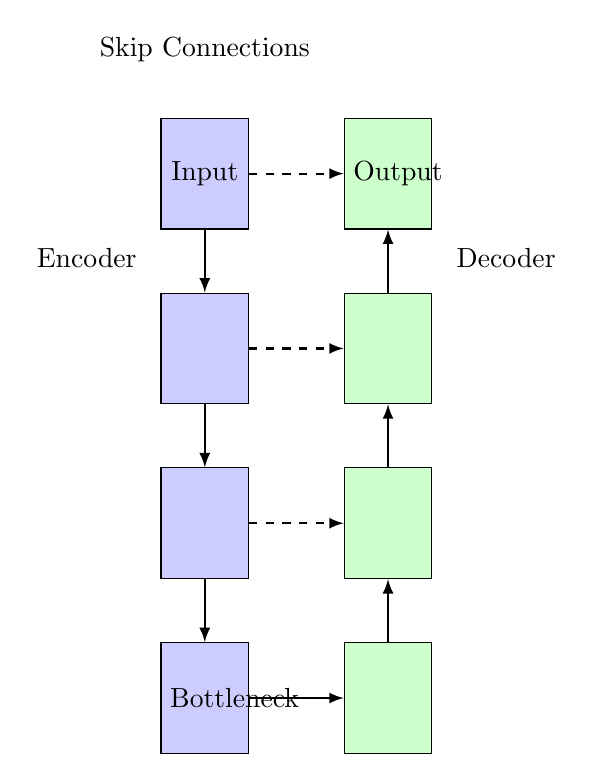
\begin{tikzpicture}[
    node distance=0.8cm and 1.2cm,
    block/.style={rectangle, draw, fill=blue!20, text width=2.5em, text centered, minimum height=4em},
    dblock/.style={rectangle, draw, fill=green!20, text width=2.5em, text centered, minimum height=4em},
    arrow/.style={-latex, thick}
]
    % Encoder Path
    \node[block] (e1) {Input};
    \node[block, below=of e1] (e2) {};
    \node[block, below=of e2] (e3) {};
    \node[block, below=of e3] (e4) {Bottleneck};

    % Decoder Path
    \node[dblock, right=of e4] (d4) {};
    \node[dblock, above=of d4] (d3) {};
    \node[dblock, above=of d3] (d2) {};
    \node[dblock, above=of d2] (d1) {Output};

    % Connections
    \draw[arrow] (e1) -- (e2);
    \draw[arrow] (e2) -- (e3);
    \draw[arrow] (e3) -- (e4);
    \draw[arrow] (e4) -- (d4);
    \draw[arrow] (d4) -- (d3);
    \draw[arrow] (d3) -- (d2);
    \draw[arrow] (d2) -- (d1);

    % Skip Connections
    \draw[arrow, dashed] (e3.east) to [out=0, in=180] (d3.west);
    \draw[arrow, dashed] (e2.east) to [out=0, in=180] (d2.west);
    \draw[arrow, dashed] (e1.east) to [out=0, in=180] (d1.west);
    
    % Labels
    \node[above=0.2cm of e2, xshift=-1.5cm, align=center] {Encoder};
    \node[above=0.2cm of d2, xshift=1.5cm, align=center] {Decoder};
    \node[above=0.1cm of d2, midway, yshift=1.2cm] {Skip Connections};

\end{tikzpicture}
\caption{A simplified diagram of the U-Net architecture, showing the symmetric encoder-decoder pathways and the skip connections that merge high-resolution features from the encoder with upsampled features in the decoder.}
\label{fig:unet_architecture}
\end{figure}


To further enhance the quality of segmentation outputs, Conditional Random Fields (CRFs) are frequently employed as a post-processing step for CNN-based methods. The integration of CRFs serves to refine the initial pixel-level predictions, with a particular focus on sharpening object boundaries and enforcing greater spatial consistency across the segmentation map. These probabilistic models achieve this by explicitly considering the spatial relationships between neighboring pixels, which helps to eliminate noise and ultimately produce results that are both more accurate and more visually coherent.

\section{Challenges and Future Directions}
\label{sec:challenges}

\subsection{Limited Training Data}
Even with considerable progress in data augmentation and transfer learning, the fundamental problem of limited labeled training data continues to be a major bottleneck in remote sensing image classification \cite{zhu2017deep}. The process of acquiring high-quality labels for remote sensing data is inherently expensive and protracted, demanding significant manual effort from domain experts \cite{xia2017aid}.

To mitigate this data scarcity issue, self-supervised learning has emerged as a particularly promising paradigm. The central idea is to learn powerful feature representations directly from large quantities of unlabeled data. This is achieved by devising "pretext" tasks, such as predicting image rotations, applying contrastive learning objectives, or reconstructing masked portions of an image, all of which encourage the model to learn meaningful semantic features without any human-provided labels.

In a related vein, weakly supervised and semi-supervised learning methods offer another avenue for reducing the annotation burden \cite{zhang2016weakly}. These approaches are designed to leverage cheaper, less precise forms of supervision, such as image-level tags or coarse-grained annotations. By strategically combining a small, accurately labeled dataset with much larger volumes of weakly labeled data, these methods can often achieve performance that is competitive with fully supervised techniques, but at a fraction of the labeling cost.

\subsection{Computational Efficiency}
The escalating size and intricacy of modern CNN models create significant hurdles for their practical deployment, especially in resource-constrained settings like satellites or edge devices. Therefore, the development of efficient model architectures and optimization strategies is not just beneficial, but essential for the widespread adoption of these technologies in real-world remote sensing applications.

A variety of model compression techniques have been developed to address this issue. These methods, which include pruning, quantization, and knowledge distillation, are designed to shrink the model's size and reduce its computational footprint while striving to maintain a high level of performance. Such approaches function by systematically removing redundant parameters or by creating more compact model representations, thereby enabling their use on platforms with limited memory and processing power.

In parallel, neural architecture search (NAS) offers a more automated solution to this challenge. NAS algorithms can systematically explore a vast design space to discover highly efficient network architectures that are expressly optimized for specific hardware limitations and performance targets. This automated design process often yields novel architectural patterns that can outperform manually designed models while simultaneously adhering to strict computational budget constraints.

\subsection{Multi-modal Data Fusion}
Modern remote sensing platforms are capable of capturing a rich tapestry of data across multiple modalities, including optical imagery, synthetic aperture radar (SAR), LiDAR, and hyperspectral sensors \cite{zhu2017deep}. However, the effective and synergistic fusion of information gleaned from these diverse sources remains a formidable technical challenge.

The most straightforward strategies are often referred to as early fusion. These approaches combine multi-modal data at the raw input level, a common example being the simple concatenation of data from different sensors. While conceptually simple, these methods necessitate the careful spatial alignment of all data sources and can struggle when faced with varying spatial resolutions or the absence of a particular data modality.

At the other end of the spectrum are late fusion methods. In this paradigm, each data modality is processed independently by a separate network branch, and the resulting predictions are only combined at the final decision level. A key advantage of this approach is its inherent robustness to missing modalities, but a potential drawback is its failure to capture intricate, low-level relationships that may exist between the different data streams.

Seeking a middle ground, intermediate fusion approaches aim to combine features at various mid-points within the network's architecture. This strategy allows for a more sophisticated and hierarchical integration of multi-modal information. These more advanced methods often employ techniques such as attention mechanisms or explicit cross-modal interaction layers to dynamically model the complex interdependencies between different data modalities, leading to a richer and more comprehensive feature representation.

\subsection{Interpretability and Explainability}
The "black-box" characteristic of many deep learning models poses a significant challenge, particularly for high-stakes remote sensing applications where understanding and trusting the model's reasoning is paramount. Consequently, the development of interpretable and explainable AI techniques has become an essential line of research for building confidence in and providing transparency for these complex systems.

A primary avenue of exploration involves visualization techniques. Methods such as activation mapping, saliency maps, and class activation mapping are designed to visually identify which specific regions within an image most heavily influence the model's final prediction. By offering these glimpses into the model's internal workings, such approaches can provide valuable insights into its behavior and help to diagnose potential biases or failure modes.

Interestingly, attention mechanisms serve a dual purpose in this context. While they are often integrated to boost model performance, they also offer a natural form of interpretability. The attention weights themselves can be visualized as a heatmap, providing a clear indication of where the model is "looking" or what it is focusing on when it makes a particular decision.

Moving toward a more human-centric understanding, concept-based explanation methods seek to identify the high-level, human-understandable concepts that a model uses to inform its predictions. By bridging the gap between abstract, low-level features and a vocabulary that humans can readily comprehend, these approaches can help stakeholders verify that a model is indeed using appropriate and sensible features for its decision-making process.

\begin{figure}[htbp]
\centering
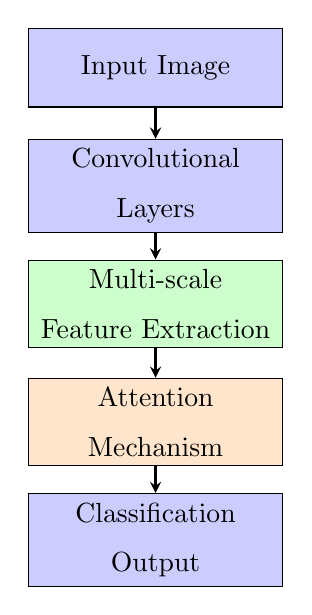
\begin{tikzpicture}[
    node distance=1.5cm,
    box/.style={rectangle, draw, fill=blue!20, text width=3cm, align=center, minimum height=1cm},
    arrow/.style={->, >=stealth, thick}
]
    % Input layer
    \node[box] (input) {Input Image};
    
    % Feature extraction
    \node[box, below of=input] (conv) {Convolutional Layers};
    
    % Multi-scale features
    \node[box, below of=conv, fill=green!20] (multiscale) {Multi-scale Feature Extraction};
    
    % Attention mechanism
    \node[box, below of=multiscale, fill=orange!20] (attention) {Attention Mechanism};
    
    % Classification
    \node[box, below of=attention] (output) {Classification Output};
    
    % Arrows
    \draw[arrow] (input) -- (conv);
    \draw[arrow] (conv) -- (multiscale);
    \draw[arrow] (multiscale) -- (attention);
    \draw[arrow] (attention) -- (output);
\end{tikzpicture}
\caption{General architecture of deep learning models for remote sensing image classification}
\label{fig:architecture}
\end{figure}

\section{Conclusion}
\label{sec:conclusion}

This paper has offered a wide-ranging review of the recent and rapid progress in the application of deep learning to remote sensing image classification, with a particular emphasis on developments that have occurred between 2020 and 2023. Throughout this review, we have delved into pivotal enhancements in CNN architectures, innovations in training methodologies, and various application-specific adaptations that have collectively propelled significant performance gains across the field.

Our examination brings several key trends and consequential developments to the forefront. It has become clear that multi-scale feature extraction techniques are now indispensable for effectively handling the vast range of object scales inherent in remote sensing data. Similarly, the integration of attention mechanisms has proven to be a highly effective strategy for enabling models to focus on the most discriminative regions and features within complex scenes. To combat the persistent issue of data scarcity, transfer learning and domain adaptation approaches have provided crucial leverage. Furthermore, the push towards lightweight network designs has been instrumental in enabling the deployment of these powerful models on resource-constrained platforms.

However, in spite of this clear progress, a number of significant challenges remain on the horizon. The availability of labeled training data, while improving, still acts as a major constraint on performance, especially for highly specialized applications or for data from emerging sensor technologies. The stringent computational efficiency requirements of many operational environments continue to present deployment challenges. Looking forward, the methods for multi-modal data fusion require further refinement to unlock the full potential of integrating information from diverse sensor suites. Finally, the crucial issues of model interpretability and explainability remain at the forefront, as building trust in the decisions of these complex deep learning systems is a vital consideration for their widespread acceptance and use.

\begin{table}[htbp]
\centering
\caption{Comparison of Deep Learning Approaches for Remote Sensing}
\label{tab:comparison}
\begin{tabular}{@{}llll@{}}
\toprule
\textbf{Method} & \textbf{Strength} & \textbf{Limitation} & \textbf{Best Use Case} \\ 
\midrule
CNN-based & High accuracy & Large data needed & Scene classification \\
Attention-based & Feature selection & Computational cost & Complex scenes \\
Lightweight & Efficiency & Lower accuracy & Edge deployment \\
Multi-modal & Rich information & Data alignment & Fusion tasks \\
\bottomrule
\end{tabular}
\end{table}

Looking ahead, several research avenues appear particularly fruitful. Further exploration of self-supervised learning is critical for better leveraging the vast archives of unlabeled data. A continued focus on efficient model design is necessary for broadening the scope of deployment on resource-constrained devices. There is also a clear need for more advanced multi-modal fusion techniques and for more robust methods that improve model interpretability. Moreover, a synergistic integration of modern deep learning with traditional remote sensing processing techniques, as well as the incorporation of explicit domain knowledge, holds promising opportunities for future breakthroughs.

As remote sensing technology continues its rapid evolution, generating ever more voluminous and complex datasets, deep learning is poised to play an increasingly central role in the extraction of meaningful information and actionable insights. Therefore, the continued and dedicated development of specialized architectures and techniques, tailored specifically for the unique challenges of remote sensing applications, will be absolutely essential for navigating the growing opportunities and complexities that define this dynamic field.


\bibliographystyle{IEEEtran}
\begin{thebibliography}{8}

\bibitem{zhu2017deep}
Zhu, X. X., Tuia, D., Mou, L., et al. (2017). Deep learning in remote sensing: A comprehensive review and list of resources. \emph{IEEE Geoscience and Remote Sensing Magazine}, 5(4), 8-36.

\bibitem{cheng2016survey}
Cheng, G., and Han, J. (2016). A survey on object detection in optical remote sensing images. \emph{ISPRS Journal of Photogrammetry and Remote Sensing}, 117, 11-28.

\bibitem{xia2017aid}
Xia, G. S., Hu, J., Hu, F., Shi, B., Bai, X., Zhong, Y., and Lu, X. (2017). AID: A benchmark data set for performance evaluation of aerial scene classification. \emph{IEEE Transactions on Geoscience and Remote Sensing}, 55(7), 3965-3981.

\bibitem{maggiori2017end}
Maggiori, E., Tarabalka, Y., Charpiat, G., and Alliez, P. (2017). Convolutional neural networks for large-scale remote-sensing image classification. \emph{IEEE Transactions on Geoscience and Remote Sensing}, 55(2), 645-657.

\bibitem{zhang2016weakly}
Zhang, F., Du, B., Zhang, L., and Xu, M. (2016). Weakly supervised learning based on coupled convolutional neural networks for aircraft detection. \emph{IEEE Transactions on Geoscience and Remote Sensing}, 54(9), 5553-5563.

\bibitem{liu2019learning}
Liu, Y., Chen, X., Wang, H., Ye, Z., Lin, Z., and Yu, P. S. (2019). Deep learning for pixel-level remote sensing data analysis: A review. \emph{ISPRS Journal of Photogrammetry and Remote Sensing}, 150, 1-15.

\bibitem{zeng2018improving}
Zeng, D., Chen, S., Chen, B., and Li, S. (2018). Improving remote sensing scene classification by integrating global-context and local-object features. \emph{Remote Sensing}, 10(7), 734.

\bibitem{deng2017enhanced}
Deng, Z., Sun, H., Zhou, S., Zhao, L., Lei, H., and Zou, H. (2017). Multi-scale object detection in remote sensing imagery with convolutional neural networks. \emph{ISPRS Journal of Photogrammetry and Remote Sensing}, 130, 83-94.

\end{thebibliography}

\end{document}